\documentclass[10pt,a4paper]{article}

\usepackage[margin=1.05in]{geometry}
\usepackage{setspace,amsmath,amssymb,amsthm}
\usepackage{graphicx,enumitem,titlesec,fancyhdr,microtype,booktabs}
\usepackage{hyperref}
\graphicspath{{../../drawings/pass2/}{../../drawings/pass1/ngon/}}
\hypersetup{colorlinks=true,linkcolor=black,urlcolor=black,citecolor=black}

\titleformat{\section}{\normalsize\bfseries}{}{0em}{}
\titlespacing*{\section}{0pt}{1.35em}{0.5em}

\theoremstyle{plain}
\newtheorem{proposition}{Proposition}
\theoremstyle{definition}
\newtheorem{definition}{Definition}
\theoremstyle{remark}
\newtheorem{observation}{Observation}

\setstretch{1.14}
\pagestyle{fancy}
\fancyhf{}
\fancyhead[L]{\small\itshape Elements of Position}
\fancyhead[R]{\small\itshape IV.\ Meetings}
\fancyfoot[C]{\small\thepage}
\renewcommand{\headrulewidth}{0pt}

\begin{document}

\begin{center}
\vspace*{1.8em}
{\large Elements of Position}\\[1.4em]
{\LARGE\bfseries IV.\ Meetings}\\[0.4em]
{\small A's spokes meet B's ratio. The docking has a closed form.}\\[1.4em]
{\normalsize Justin Erholtz}\\[0.3em]
{\small 24 September 2026}
\end{center}

\vspace{1.0em}

\begin{center}
{\large \(2\) is named by \(1\).}
\end{center}

\vspace{0.8em}

\noindent
\textit{A note.}
Part~I named the pair.
Part~II walked one street and split two mixes.
This part lays a second street on the same midline and measures the meetings.
Tables cited live under
\texttt{kernels/ngon/runs/2026-09-24\_n1-60/} and
\texttt{measures/bridge/runs/2026-09-24/}.

\tableofcontents

\section{Named by one}

\(1\) names \(2\) by inverting the primary cut of Part~I:
\(2=1/(1/2)\).
On the pair \((x,2-x)\) the arithmetic mean is constantly \(1\), and equals the geometric mean only at \(x=1\).

The second street is not a new unit.
It is the same unit asked the other way.
After arrival it walks back toward the lock.
Call the outward integer count street~A and the inward golden walk street~B, once, and then use the marks.

\section{The common object is the line}

The common object is not a circle.
It is the \(1/2\) line.

Every local diameter is cut at its midpoint.
Street~A's even split lives there.
Street~B's pair \(\varphi\) and \(1/\varphi\) lives equally far from it.
The cone of A, height the count, has slope \(1/2\).

Freeze \(n\): an \(n\)-gon of diameter \(n\), a half-walk, a \(\varphi\) mark, an inward copy of radius \((n/2)/\varphi\).
All of that is a section.
Start the count and the same marks ride A outward and, after arrival, walk B the other way.

\section{Marriage at five}

\begin{proposition}
\[
2\cos(\pi/5)=\varphi.
\]
\end{proposition}

The n-gon kernel writes this as column \texttt{twocos} of \texttt{rings.csv}.
On the \(24\)~September run, at \(n=5\),
\[
\texttt{twocos}=1.618033988749895,
\]
difference from \(\varphi\) equal to \(0\) at double precision.

The same five, asked of the walk by the vertex mix \(h=\tan(2\pi/5)\):
one elementary step per vertex, max error \(4.44\times 10^{-16}\), closing distance \(3.4\times 10^{-17}\), five unit sides equal to \(2\sin(\pi/5)\) with error \(0\).

That is the bridge row \(n=5\).
A's own split at five \emph{is} B's ratio, and the walk at the vertex mix \emph{is} the pentagon.


\begin{figure}[htbp]
\centering
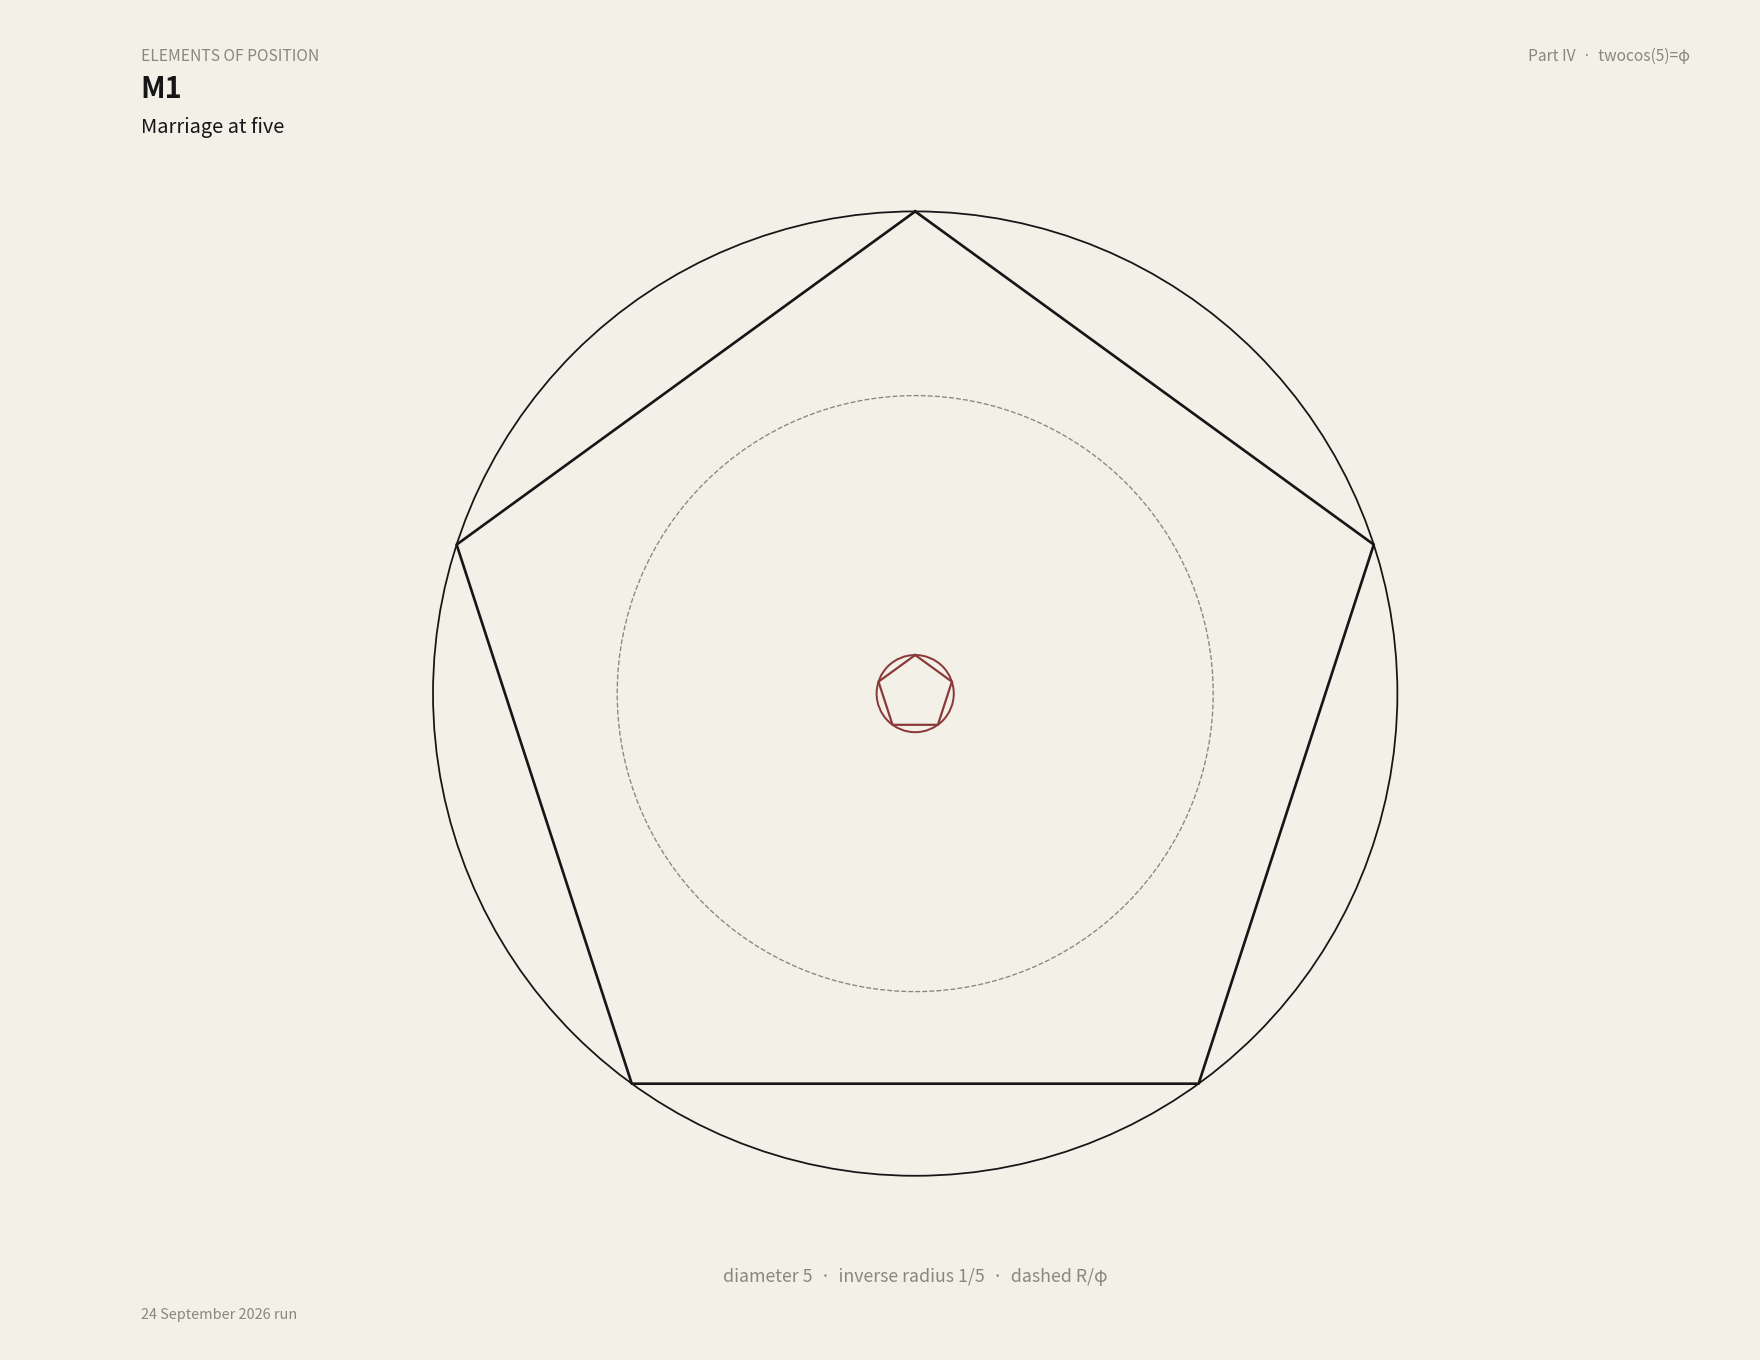
\includegraphics[width=0.92\textwidth]{M1_marriage.png}
\caption{Sheet M1. Regular $5$-gon of diameter $5$. Dashed inward copy at $R/\varphi$. Accent is the inverse locus of radius $1/5$.}
\end{figure}

It does not spread to a generic later integer.
It is not the half-turn mix.
The half-turn mix at \(n=5\) is \(h=\tan(\pi/5)\), one gap letter \(5\).
The vertex mix at \(n=5\) writes gaps \(\{2,3\}\).
Both are true.
They are two kicks.

At the recorded grain \(h=0.002\), placing the same pentagon by walking rounded fractions of \(2H\) steps on a circle of diameter \(5\) leaves a visible miss: max angle error \(0.00145\), max side error \(0.00292\).
Spokes remain \(2.5\).
That miss is Part~III's residual, not a failed marriage.

\section{Docking}

Fibonacci docking is a different kind of meeting: approximate, after arrival, shrinking as the count runs.

\begin{proposition}
\(F_k\varphi-F_{k-1}=-\psi^{k}\) exactly, where \(\psi=(1-\sqrt5)/2\).
The docking error is
\[
\frac12\bigl|F_k\varphi-F_{k-1}\bigr|=\frac{1}{2\varphi^{k}}.
\]
\end{proposition}

\begin{observation}
At \(k=7\) (\(N=F_7=13\)), \(1/(2\varphi^{7})=0.0172209\), matching the older printed ``about \(0.017\).''
At \(k=13\) (\(N=233\)), \(1/(2\varphi^{13})=0.0009597\), matching ``about \(0.00096\).''
\end{observation}

Cassini's identity is the case \(M=RL\) of unimodularity on the Stern--Brocot tree.
The identical mechanism with \(\delta=1+\sqrt2\) gives a Pell analogue whose conjugate is smaller than \(1/\varphi\), so that docking, were it built, would converge strictly faster.
It is not built here.


\begin{figure}[htbp]
\centering
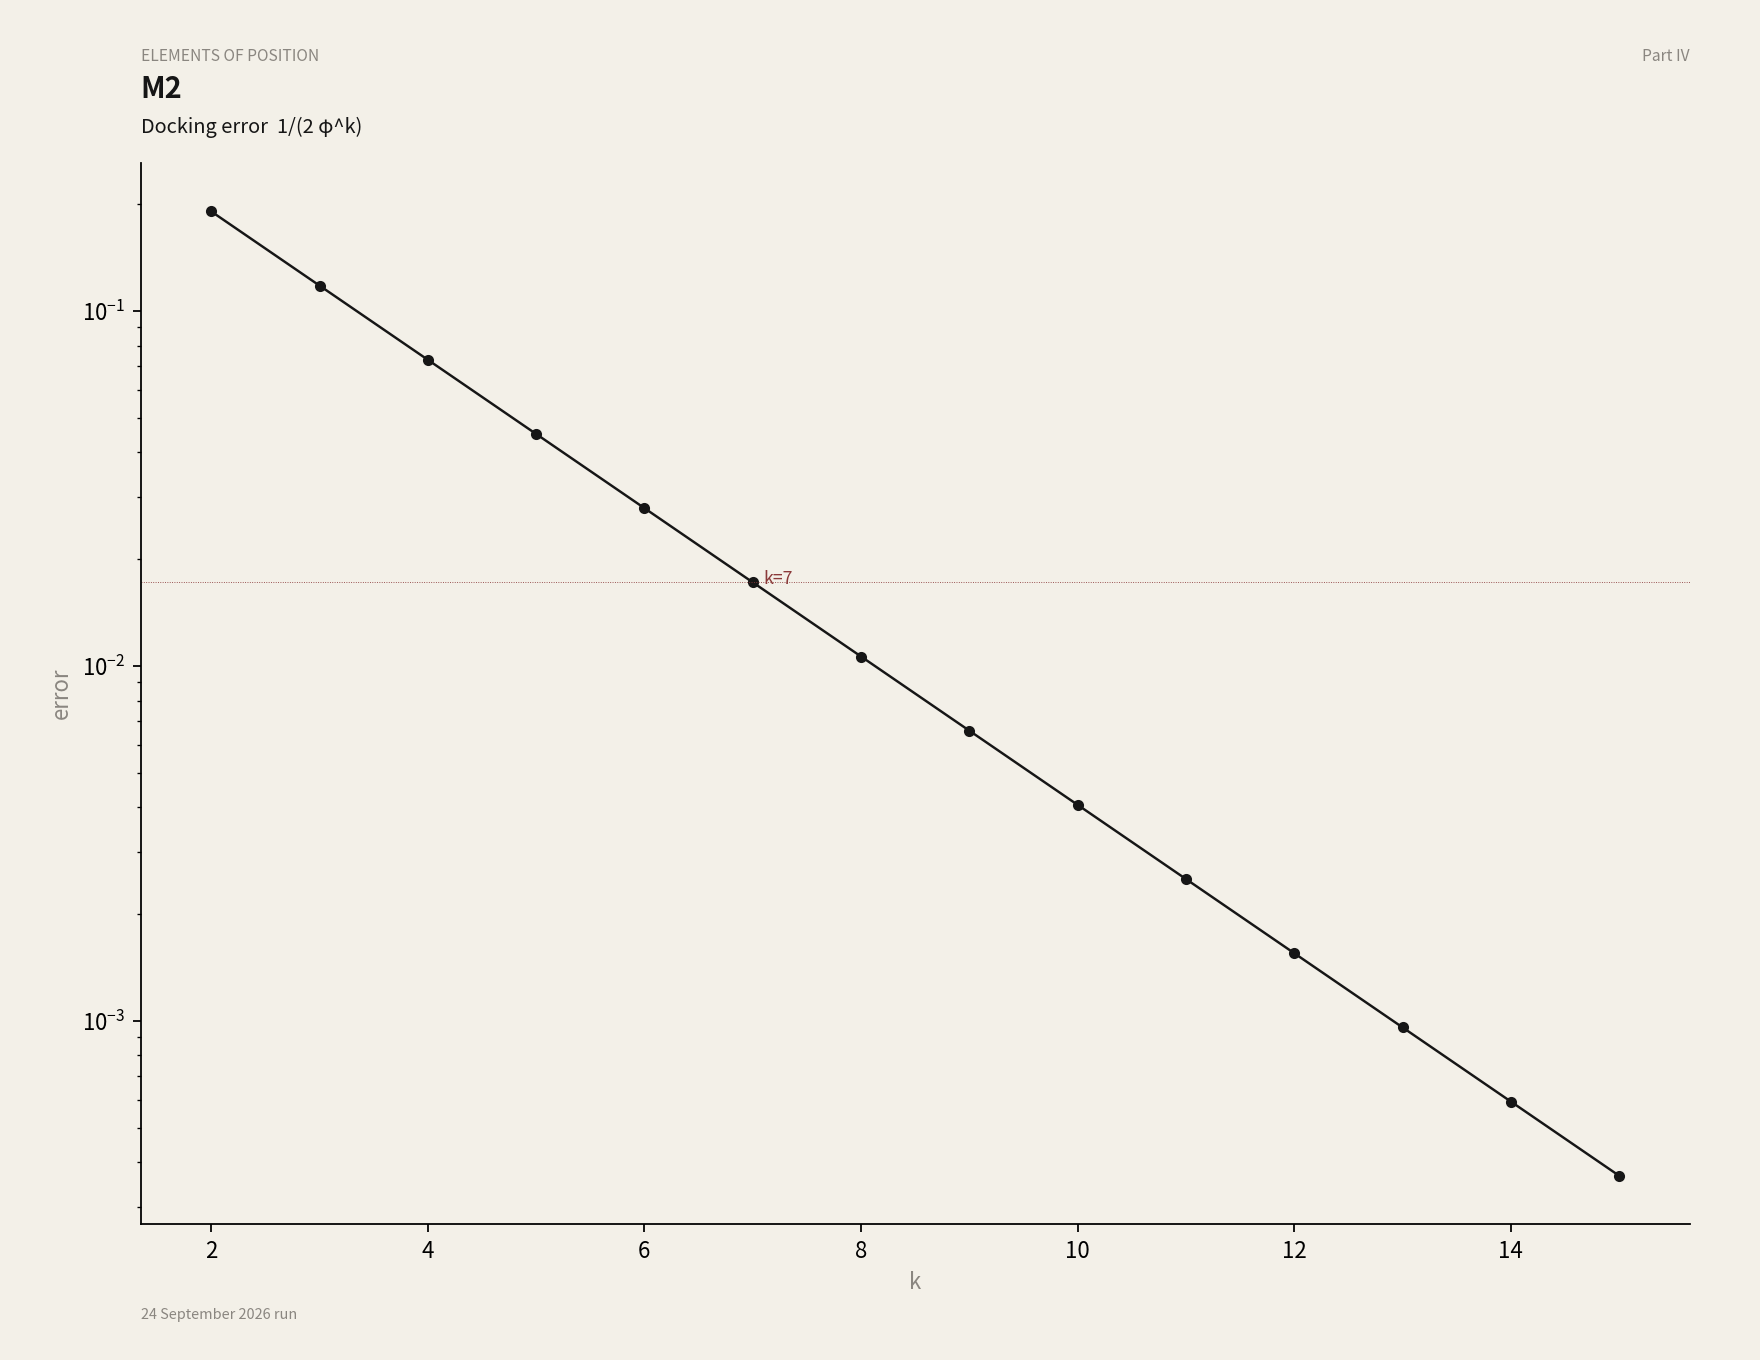
\includegraphics[width=0.92\textwidth]{M2_docking.png}
\caption{Sheet M2. Docking error $1/(2\varphi^k)$. The mark at $k=7$ is the old printed $0.017$.}
\end{figure}

\section{What stands}

Forced:
\(2\) named by \(1\);
the \(1/2\) line as the common object;
marriage at five, two routes, machine agreement on the \(24\)~September tables;
docking error \(1/(2\varphi^{k})\).

Not granted:
marriage at a generic integer;
the vertex mix spoken as if it wrote one gap letter \(n\);
a numeric relation between \(\gamma\) and \(\varphi\).

Where is \(1\)?
It is the lock both streets still share.

\end{document}
